\chapitre{Les errements nyctalopes d’une grande folle, du 22 au 25 juillet 2033}{Etre gai à Rimouski,}{ ce n’est pas l’être à San Francisco, à Vancouver ou à Montréal. À Rimouski, il n’y a pas de «village», la communauté étant étalée un peu partout dans les quartiers, dans les paroisses limitrophes et dans les petites villes avoisinantes. Il n’y a ni sauna, ni salon de coiffure, ni sex shop pour homosexuels. Si certains bars sont plus gais que d’autres, les clients «straights» y sont quand même omniprésents. Les épais également. D’où les deux heures de musculation et de boxe que s’impose Shimoune Saint-Pierre quatre ou cinq fois par semaine, si ce n’est pas plus. C’est ce qui explique pourquoi ses tenues extravagantes, voire fofolles, contrastent avec le diamètre imposant de ses biceps et la forme inquiétante de ses poings. }

Si d’aventure, il doit défendre son personnage qu’un idiot choisit bêtement d’agresser, il s’en tire toujours sans une égratignure, sauf peut-être certaines rougeurs sur les jointures après avoir fracturé un nez, ouvert une arcade sourcilière ou disloqué une mâchoire. Sa philosophie de base se résume ainsi : «Simoune oui, moumoune, non !» 

Il en est des gais comme des hétéros. Les gens sont normalement d’un ennui mortel; leur quotidien est routinier, insipide, assommant, mécanique, déprimant. Pour se désennuyer, ils regardent, de leur salon, de leur terminal, de leur télé, de leur coin de fenêtre sur la rue Crouet, la vie d’une poignée de marginaux qui eux, artistes, sportifs, malfaiteurs et autres vedettes, bourlinguent à fond la caisse. Ils la commentent et l’analysent, cette vie qu’ils épient. Ils l’aiment ou la détestent. Ils rêveront souvent de pouvoir se l’offrir, de pouvoir ainsi rechercher les sensations fortes, les histoires folles, les sauteries prodigieuses, les partouzes démentielles, les rencontres inoubliables, les voyages au bout de soi, les raids au bout de la nuit, les intoxications par substances légales ou non, les moments puissants et les souvenirs inaltérables.

L’ami Saint-Pierre, lui, il est un gai vivant. Très vivant ! Mais sauf exception, il est plutôt raisonnable durant la semaine; pourquoi indisposer inutilement son patron Amédée Chicot en entrant au boulot avec une tête de zombie, des yeux de poisson mort et l’intérieur de la bouche en plancher d’écurie ? Par contre, le vendredi soir, dès son quart de travail terminé, il va se mettre à l’affût de «gros partys débiles» et s’il en trouve, zou!, il va tout faire pour fracasser son record personnel de dérape. On n’a qu’une vie, non ? En revanche, si rien ne se passe, il va se changer les idées en alternant sa fin de semaine entre chez lui et le gymnase. Chez lui, il fera du ménage, écoutera de la musique et préparera de la bouffe, au gym il suera et gardera un œil ouvert sur les occasions. Surtout aux douches.

Quand en début de soirée, il a fait son entrée - remarquée comme toujours - à l’Errance, un bar huppé du quartier Saint-Germain, il a immédiatement repéré son ami Martin «Tintin» Arsenault, un collègue de la jaquette délirante, qui buvait du champagne avec un quinquagénaire porteur de fringues que seuls les moralement pourris qui sont socialement acceptables peuvent s’offrir. Son cerveau s’est alors mis en mode SQL et, en quelques secondes, il a identifié le bonhomme comme étant un comptable agréé de Sainte-Luce associé au parti Liberal, un dénommé Jonathan Roy. Bon père de famille, notable apprécié dans son village de banlieue, il lui arrivait parfois de venir s’acoquiner avec de jeunes hommes de Rimouski, question d’assouvir les plus secrets de ses fantasmes.

Comme Tintin lui a fait signe, Shimoune s’est approché et s’est fait offrir une coupe. Puis il y en a eu d’autres. Subodorant un potentiel d’agapes, il s’est accroché et, au bout de deux heures, c’est-à-dire quatre bouteilles de Veuve, il s’est retrouvé ami de longue date de Roy, qui, plus ivre que pompette, s’est dit prêt à passer à du plus costaud, du moins cucul.

Shimoune le regarde dans les yeux.

- Genre ?

- Genre que j’appelle un ami et qu’on se fait inviter à son party. Un b’en gros party dans une grosse cabane au Bic en face du fleuve. Y a jamais de trous du cul, seulement du monde qui ont de l’argent. On a l’astie de paix.

- Quelle sorte de monde, mon Jon ?

- Du monde qui aime la vie.

\begin{floatingfigure}[l]{50mm}
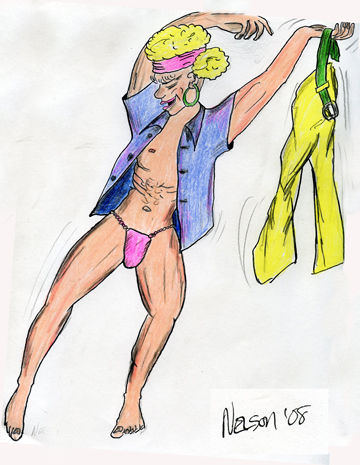
\includegraphics[height=60mm]{corps/chapitre13/img/personnage-simonstrip.jpg}
\end{floatingfigure}

Tout un euphémisme pour décrire une trentaine de bourgeois, hommes et femmes, gais, lesbiennes, hétéros, fétichistes, échangistes, exhibitionnistes et autres dépravés, n’ayant en commun que l’appartenance au parti libéral et l’argent. Beaucoup d’argent. Beaucoup plus qu’il n’en faut pour bien faire comprendre à ceux ou celles qui s’aviseraient de vouloir cancaner sur ces activités sulfureuses, qu’ils ou qu’elles le regretteraient toute leur vie quelle qu’en soit la longueur résiduelle.

La partouze a pour cadre une très grande maison construite il y a quinze ans, une construction où les matériaux dominants sont le chêne, l’érable, le cerisier et la pierre, dont les plafonds sont à douze pieds et qui s’enorgueillit d’une longue véranda vitrée et chauffée faisant face au fleuve. Pour y accéder, on doit quitter la 132 à la baie Hâtée, à l’est du village du Bic. De là, un mauvais chemin de terre serpente vers le nord jusqu’à la voie ferrée, la traverse dangereusement et continue en direction ouest pendant un kilomètre. Un stationnement asphalté apparaît alors où, ce soir, une quinzaine de voitures horriblement chères sont alignées.

Shimoune qui n’a pas assez de doigts pour compter les chambres dans le plain pied décoré de toiles, de sculptures et de tapisseries anciennes, remarque ici et là, de petites soucoupes d’argenterie pleines de cocaïne, de grands crus ouverts un peu partout, un bar étourdissant dont la spécialité semble être le scotch, des cabarets d’amuse-gueules où le caviar russe a vraiment été privilégié, une projection holographique de deux lesbiennes en train de s’aimer charnellement et deux immenses foyers hybrides à combustion contrôlée où des brasiers d’érable combattent la fraîcheur fluviale de cette douce soirée de juillet. Le mur ouest du vaste salon est une verrière donnant sur une piscine où quelques baigneurs batifolent, verre en main, dans leur plus simple appareil.

Si la plupart des gens sont habillés, certains portant des kimonos en ratine blanche, quelques-uns, pas nécessairement les plus beaux, sont nus. On s’embrasse, on se caresse, on se sourit, on s’esclaffe, on se raconte des trucs. On est seul comme cet exhibitionniste qui circule partout, le braquemart même pas au garde-à-vous, en duo comme ces fétichistes hautement bottés qui sont venus en moto, en triplet comme ce couple arrivé en compagnie d’une jeune fille du type voluptueux - Shimoune la reconnaît comme étant une des adjointes administratives de Carl Michaud, mais se garde bien d’aller la saluer – ou en quatuor comme ces deux couples échangistes qui éprouvent toutes les misères du monde à embrayer tellement l’une des deux paires est peu appétissante. Ce qu’on parvient à faire l’est au vu et au su de tous, ce qui contribue au climat général de la petite fête.

Avant que ne se présente à lui cette femme extraordinairement belle et svelte, la seule à porter un kimono noir, Shimoune, la Grande folle du manger mou, se sera adonné à différents exercices. Tout d’abord, à un indicible effeuillage au terme duquel ce qui lui sert de bobettes aura abouti, deux mètres plus loin, sur l’incontestable évidence d’un sérieux cas de priapisme. Ensuite, il se sera investi dans une session très applaudie de lutte gréco-romaine, calibre «jeux gais», où il aura pu récupérer son soi-disant slip, son adversaire étant l’infortuné porteur dudit cas de priapisme. Quant aux autres activités, contentons-nous d’imaginer qu’elles correspondaient à sa définition de «gros party débile» !

Il vient à peine de porter à ses narines une petite cuillère de poudre blanche, que la blonde, tout en grâce et en dignité, s’approche, les deux mains dans ses cheveux coupés à la nuque. De ses grands yeux verts, elle regarde Shimoune, la tête un peu inclinée. Si elle est saoule, rien n’y paraît et si elle est cokée, son calme le cache parfaitement. Elle lui déclare le trouver «magnifique et appétissant», même s’il n’est «pas complètement déshabillé», même s’il semble passablement éméché. Lentement, elle caresse, de ses longs doigts manucurés, les marques de lutte qu’il s’est infligé dans le haut des bras et, sans aucune retenue, lui annonce dans un français germanisé qu’elle souhaiterait qu’il lui «fasse des choses». Quand il lui confesse son orientation sexuelle, une condition à laquelle il n’a jamais pu déroger, elle n’insiste pas et, sans mot dire, on la dirait résignée, habituée à la fatalité, l’amène par la main jusqu’à l’autre bout du salon. Un pansu aux épaules en bouteilles semble l’attendre depuis le divan de cuir où il est langoureusement étendu.

- Ché fous présente mon mari, le propriétaire de la maison. Ça fait cinq ans qu’il ne m’a pas baisé; il ne s’intéresse plus qu’aux hommes. Moi, ché mé démerde comme ché peux. Allez, ché fous laisse, auf wiedersehen.

Shimoune connaît ce peu appétissant mollasson. C’est Pete Barrett, Pierre Barrette dans ses jeunes années, l’homme du pouvoir libéral occulte dans la région. Tout passe par ses petits doigts boudinés et sans lui, le gros Turcotte ne serait rien. On dit de cette limace baveuse qu’il n’a pas d’amis, mais qu’il est suicidaire de s’en faire un ennemi. On chuchote que Philippe Dauphin et Carl Michaud lui doivent leur poste. Idem pour cette enflure d’Amédée Chicot, le patron du centre nutritionnel.

Il est inutile ici de préciser la suite immédiate de cette rencontre. Disons, pour résumer, que malgré son état compliqué, abscons, brumeux, Shimoune pourra témoigner du fait que contrairement à ce que peut laisser croire sa dégaine obèse de puissant patapouf décadent, Barrett passera rapidement aux actes, ne s’en tiendra qu’aux actes, c’est-à-dire qu’il ne sera jamais passif au sens receveur du terme, et se montrera d’une patience vicelarde jusqu’à ce que Shimoune arrive à contrecarrer avec de sérieux rugissements, le handicap dont l’avait frappé le cocktail polytoxique absorbé depuis le début de la soirée.

À son étonnement, le gastéropode lui fait signe que c’est terminé et qu’il ne s’attend pas à se faire rendre la politesse. Presque en même temps, comme si elle avait été aux aguets, la blonde revient le chercher.

- Si fous sêtes intelligent, fous ne répéterez à perzône, entendez-fous, à perzône, qu’il zouffre de dysfonction érectile chronique. Si jamais fous parlez, si jamais fous le dites à quelqu’un et qu’il l’apprend, il fa fous faire regretter le jour de fotre naissance. Il est tré doué pour ceula.

Elle ouvre alors son kimono et, l’espace d’un instant, dévoile une vilaine cicatrice rougeâtre qui lui balafre le ventre des seins jusqu’au pubis.

- Fous savez compris ?

Shimoune en a la chair de poule. Quel porc ! Il fait jouer la rabatteuse pour impuissants à cette magnifique Allemande, ensuite il lui fait faire le panneau avertisseur.

Quelques mètres plus loin, Tintin semble en avoir fini avec Jonathan Bérubé. Le bonhomme est couché par terre et ronfle comme un quanticordi dont le ventilateur est en train de sauter.

- C’est du vin à 250 \$ la bouteille, dit-il à Shimoune , un Château Balestard à bout de bras.

- Amène-le, on va le finir. Moi ici, j’ai un Château Clément Pichon, ça doit pas se donner ça non plus.

Les deux compères se rhabillent et décident de sortir avec leur pinard de millionnaire. Le jour est en train de se dégourdir de sa nuit, les chauves-souris sont retournées se suspendre à leur plafond, les oiseaux les moins paresseux ont déjà amorcé leur jabotage et le fleuve commence à changer de couleur. La journée sera très chaude.

- J’ai amené une soucoupe de poudre.

- J’p’us capab’, répond Shimoune qui lance son verre à bout de bras.

- D’vait b’en y en avoir pour 100 \$ !

Cette fois, c’est l’assiette qui file vers la stratosphère.

- Sais-tu ce qu’on devrait faire, continue Martin Arsenault, alias Tintin, on devrait aller marcher sur les galets au bord de la mer. Il fait tellement beau.

- OK, j’te suis.

La dentelle côtière d’une parfaite irrégularité qui s’étire à l’ouest vers le Bic et Saint-Fabien, n’est qu’un jeu infini de galets parfois acérés, de récifs imposants sur lesquels il faut souvent se hisser, d’anses ténues avec leurs familles de canards, de baies minuscules qui disparaissent à marée basse, de terre-pleins en caillou ou en gros sable, avec, en avant, tantôt très près, tantôt plus éloignées, des îles grandes ou petites, et, derrière, des caps et des falaises boisées dont des cèdres et des épinettes ayant poussé tout croche au travers des roches. Le fleuve y est le maître absolu avec ses vagues crémées d’écume salée, gavées de varech et de goémon arrachés, qui, en clapotant, viennent parfois lécher la grève comme s’il s’agissait d’un câlin, mais qui parfois, avec fracas, tentent de tout démolir comme si la rage du tonnerre de Dieu voulait annihiler ce paysage antédiluvien. Ici un huard méfiant, là des macreuses qui semblent ne pas comprendre ce que font, trop près d’elles, ces quelques bernaches égarées et ces familles d’eiders plongeurs, à moins que ce ne soient des macreuses. Plus loin, occupées à brailler, des mouettes que l’on croirait libérées d’un site d’enfouissement sanitaire. Et, invisibles, parce qu’il faut pouvoir prendre son temps si on veut les apercevoir et les observer, quelques loups marins rôdent en quête de leur premier festin de la matinée.

Mais en cette journée qui s’amorce, le nez vers le vent du large, Martin et Shimoune s’intéressent à peine aux oiseaux. Et vice versa, du reste. Comme la marée descend, leur expédition s’avère moins difficile. Les passages où il faut se glisser dans un demi-mètre d’eau glaciale sont presque tous en voie de se résorber. Au besoin, les deux excursionnistes du petit matin s’entraident sans devoir parler. Une main tendue suffit. On monte, on saute, on ahane, on grimpe, on reprend son équilibre, on s’arrête le temps de souffler.

- T’as vu là-bas ? Y a un oiseau qui vient de plonger.

- Ouin, c’est un balbuzard, répond Shimoune, sûr de lui.

- B’en non, y en a p’us au Bic.

- B’en ça doit être un faucon pèlerin…

- B’en non, espèce de grande folle, ça pêche pas, un faucon pèlerin.

- J’sais-t’y moi !

D’efforts en repos, de silence en débats ornithologiques, les jeunes gens finissent par aboutir à la Pointe-aux-Anglais, face au chenal séparant la terre ferme de l’île-au-Massacre. Mais puisqu’ils sont fatigués, hébétés, mouillés, devenus peu loquaces, ils décident de s’en retourner chez Pete Barrett, question de se trouver un samaritain disposé à les ramener à Rimouski. À la différence que cette fois, crevés par leur nuit inavouable, ils le feront par en haut, en empruntant l’ancien chemin de randonnée qui traverse le bois en direction est. Le point de départ est le premier de ces trois chalets insolents qui ont été construits sur la pointe au siècle dernier. Aussitôt dit, aussitôt fait ! Malheureusement, la piste n’est plus que vaguement balisée et le trajet promet d’être aussi pénible qu’à l’aller. Tintin parle même de retourner au bord du fleuve.

Or voilà qu’après avoir contourné un énorme rocher, un pavillon du même style, mais encore plus impressionnant que la maison de Barrett, apparaît presque miraculeusement dans leur champ de vision. Construite au milieu d’une éclaircie probablement volée à la forêt par l’entrepreneur, l’habitation est entourée de pelouse, de bosquets, d’arbustes et de haies. À ce qu’ils peuvent voir, la partie avant du terrain paraît mieux nantie. Il semble même y avoir un chemin d’accès asphalté avec muret d’apparat et barrière. Plus près d’eux, c’est l’arrière de la maison qui s’offre avec une baie vitrée protégeant contre les vents salins l’immense véranda qui l’habille en totalité.

Shimoune croit apercevoir quelqu’un en train de s’y affairer.

- Y a un Bon Dieu pour nous autres, s’écrit-il. Je vais aller lui demander s’il y a un chemin facile pour se rendre chez Barrett.

En s’approchant, il remarque que les bas de fenêtres ont été ouverts afin que l’air frais du matin puisse bien pénétrer par les moustiquaires. C’est ce qui lui permet d’entendre des exclamations, des rires et un certain brouhaha. Replaçant ses cheveux de folle du mieux qu’il le peut, il monte poliment l’escalier de la véranda où, constate-t-il, il n’y a plus personne. Par contre, merci aux grandes croisées de chaque côté de la porte, il voit que ce n’est pas le cas plus loin à l’intérieur. Dans ce qu’il lui apparaît comme étant une vaste salle à manger, des gens vont et viennent, des gens apparemment arrivés à un âge avancé à l’exception d’un gaillard d’aspect jovial, une sorte d’Hercule bedonnant qu’il rencontre tous les jours au rez-de-chaussée du Centre sous la forme d’une statue en bronze, le gros Turcotte lui-même. Instinctivement, le préposé au manger mou, fif de réputation, fait le mort. S’il frappe à la porte, il sera mis en présence de l’homme fort du régime libéral. Passe encore le dysfonctionnel Pete Barrett, mais l’homophobe Sylvain Turcotte c’est un peu trop lui demander ce matin.

Au moment où il va reculer prudemment pour rejoindre son compagnon dans le sous-bois, il voit le ministre s’écrier à grand renfort de gestes avant de disparaître du champ de vision :

- Papa, maman, bonyenne, arrêtez ça. Quand on fête son soixantième anniversaire de mariage, on fait pas le ménage. On reste assis et on se fait servir. Pas vrai matante Germaine ?

- Oui cher, fait une voix stridente. Ton pére p’is ta mére l’ont b’en mérité.

Turcotte réapparaît avec, bras dessus bras dessous, un vieil homme aussi énorme que lui et une vieille dame qui joue à celle qui proteste.

- Mon oncle Lucien, avez-vous crinqué vot’ violon pour la fête d’à soir ? crie, hilare, le gros Turcotte par-dessus son épaule.

- Oui mon homme, m’a te faire souigner la baraque.

Papa, maman, tante Germaine, oncle Lucien ? Qu’est-ce que c’est que ce bordel ?

- Maman, arrête de faire la baboune. Aujourd’hui, tu relaxes, c’est ta fête, à toi et à papa ! T’es quand même pas pour annoncer que tu demandes le divorce au bout de 60 ans !

Profitant des rires puissants du ministre qui semble animer, à grand effet de bide, ce qui pourrait être un petit-déjeuner, Shimoune opte pour une retraite discrète.

Une fois dans les fourrés, il fait signe à Martin de garder le silence et de le suivre sans faire de bruit. Son plan est simple, si, côté façade, il y a une voie carrossable, c’est que des voitures en provenance de la 132 peuvent venir. Donc, en contournant par le bois pendant quelques centaines de mètres, on arrivera sûrement à un chemin d’accès sans risquer d’être vu par Turcotte ou par sa parenté. De là, il sera facile de se rendre chez Barrett.

Effectivement, cinq minutes plus tard, les deux randonneurs débouchent sur la route de desserte où il ne leur reste plus qu’à marcher une quinzaine de minutes pour atteindre la section locale de Sodome et Gomorrhe. Mais ce faisant, ils auront eu le temps de constater que deux taupins montaient la garde à la barrière d’entrée chez Turcotte. À moins que ce ne soient deux employés du cabinet de Turcotte en train de prendre l’air matinal. En y songeant bien, pourquoi faudrait-il des gardiens ? Y aurait-il quelque chose à cacher ? Et si ce sont des gardiens, ils ne semblent pas très professionnels.

- Ils n’ont pas pensé qu’on pouvait arriver par le bois du côté du fleuve.

- Qui ça ?

- Les deux gardiens.

- Quels deux gardiens ?

- Ceux du gros Turcotte !

- Le gros Turcotte ?

- B’en oui, il est là-dedans avec son père, sa mère, avec des mononks, des matantes …

- Lâche la coke, ma chouette. Les parents à Turcotte sont morts dans un accident, il y a quelques années de ça. Les médias en ont fait tout un plat.

- Je te dis que je viens de les voir !

- Ouin ouin !

Ébranlé, sa fatigue étant ce qu’elle est, Shimoune n’insiste pas, pas plus qu’Arsenault du reste. Se pourrait-il qu’il ait halluciné ? L’alcool, la coke et l’effort physique en synergie ? Pourtant !

Après avoir dormi quelque dix heures en ligne, il refait surface hanté par l’image du ministre libéral. Même en avalant ses œufs bouillis, il n’arrive pas à décrocher. N’est-ce pas à cet immonde manœuvrier populiste que le Québec doit de voir ses aînés bouffer du Nutrisuz, être encagés comme des bêtes, être exterminés pour cause d’improductivité ?

Son ordinateur a beau être une antiquité du début de l’informatique quantique grand public et son affichage cruellement dépourvu de la techno nécessaire aux présentations holographiques, il permet néanmoins la navigation vocale et le traitement simultané en 3D de requêtes multiples. En prime, il sert de système musical sophistiqué. C’est donc confortablement emmitouflé dans la musique de Gilles Bélanger, celle des hommes rapaillés de Gaston Miron qui joue en boucle, que Shimoune vadrouille un petit trois heures dans le cyberespace.

Sa première découverte troublante lui provient du GRFR (Grand registre foncier régional) qui lui révèle tous les détails légaux particuliers à cet immense pavillon que fréquente ou … fréquenterait Sylvain Turcotte. Il a été érigé en 2028, l’année du référendum et de la création des CRG, il appartient à l’État et est sous la juridiction du ministère des Affaires gérontologiques (MAG).

- Bingo, la boîte du «gros verrat»!

Construit au coût de 3,4 M\$, sa valeur foncière est actuellement de 4,8 M\$, ce qui inclut un terrain de 2,2 acres et un chemin privé de 300 mètres. Puis, une cybervisite dans les pages déclaratoires sur l’affectation des ressources immobilières du MAG apprend au fouineur que le bâtiment sert aux relations publiques du ministère, en ce sens qu’on y tient parfois des sessions de travail loin de la trépidation urbaine. Son responsable est Philippe Dauphin, cadre du MAG et directeur des communications au CRG/BSL.

- ‘Stie, le Flipper !

\begin{floatingfigure}[l]{50mm}
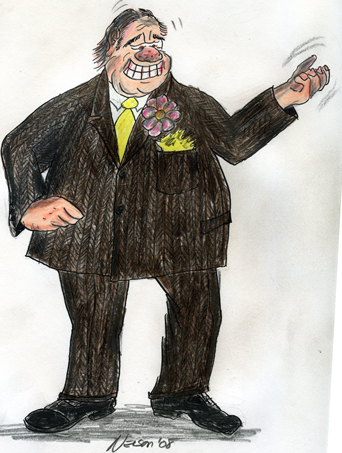
\includegraphics[height=60mm]{corps/chapitre13/img/personnage-turcotte1.jpg}
\end{floatingfigure}

Encouragé, Shimoune entreprend alors de suivre la carrière de Turcotte à la trace et, fatalement, il aboutit à cet horrible accident survenu en juin 2029 où un minibus avait fait une embardée sur la 20 à la hauteur du pont de la rivière Chaudière. Six personnes, tous membres de la famille du ministre libéral, avaient ainsi perdu la vie. Éploré, Sylvain Turcotte avait parlé de la «cruauté du sort» qui «sans préavis» privait son père, sa mère, deux de ses oncles et deux de ses tantes, «des gens modestes, sans autonomie financière même s’ils ont travaillé fort toute leur vie», de cette belle retraite qui les attendait au nouveau CRG de Rimouski, le «fleuron» du réseau institutionnel qu’il venait à peine d’inaugurer. La cérémonie funéraire avait été presque civique et les cendres avaient été éparpillées aux quatre vents sur le fleuve.

- Peuvent pas être plus morts que ça !

Et soudain, Shimoune reçoit un voyage de pierres sur le crâne. Un reportage vidéo lui présente Turcotte en compagnie de ses parents lors de la campagne référendaire de 2028. Qui plus est, Mimi Turcotte, sa mère, une femme d’allure sévère que l’on identifie comme étant la responsable régionale du recrutement des bénévoles, affirme que la campagne va très bien et qu’elle est très fière de son fils dont le projet envers les aînés va entrer dans l’histoire du Québec. Or, à quelques détails près, cette dame est exactement la même que celle qu’il a aperçue ce matin, celle qui semblait vouloir se faire tirer l’oreille. S’il avait vu juste. S’il n’avait pas halluciné. Mais depuis quand hallucine-t-on avec de la coke de riches ? Qu’est-ce que c’est que ces embrouilles ?

Et Miron de pousser dans les enceintes de Shimoune:

    - À tourmenter la nuit les vents là-haut
    les ciels poudreux d’étoiles brûlées
    où sont par ce temps mes pères et mères
    ma famille que jamais je ne revois
    et les visages peints de mes croyances

    j’erre dans la ville sans être heureux
    par rues et rafales sans hâte de dormir …

Une histoire qui n’est pas sans ressemblance avec celle des parents de son ami Timothée Tardif, une prof de musique avec un CV impressionnant et un camionneur retraité. Tous deux morts dans un incendie criminel, mais qui sont réapparus sous forme d’illégaux à la charge de leur fils. Étrange !

Une série de clips provenant de la campagne de 2019 attire néanmoins son attention. C’est le début de carrière du gros Turcotte. Il a peut-être quatorze ans de moins sur le compteur, mais il est aussi gros, aussi grand, aussi fort en gueule. Un des reportages nous le montre au sein de son comité électoral où, encore une fois, Mimi Turcotte apparaît, identifiée cette fois comme étant la directrice adjointe de l’organisation libérale du comté. On l’entend dire qu’elle a réussi à recruter des gens de qualité en provenance de tous les milieux, des artistes, des professionnels, des cultivateurs, des jeunes, des immigrants, qui viennent s’impliquer parce qu’ils sont convaincus de la plateforme progressiste et juste du candidat Sylvain Turcotte, son fils. Et parmi ces bénévoles extraordinaires qu’elle cite en exemple, elle en a justement trois près d’elle, un étudiant en sociologie, lettres et communications à de l’Université du Québec à Rimouski, Philippe Dauphin, un comptable agréé de Sainte-Luce, Jonathan Roy, et une violoncelliste de renommée mondiale, Marie Rioux.

- Attends un peu …

Shimoune aura besoin d’une quinzaine de minutes bénédictines dans les archives de l’actualité régionale avant de tomber sur l’histoire de l’incendie criminel de Saint-Anaclet. Le reportage lui semble clair. Les deux victimes sont Romain Tardif, un camionneur retraité, et Marie Rioux, la violoncelliste bien connue «dont l’incessante contribution au milieu culturel régional en fait une perte irremplaçable». Les rouages de son cerveau se mettent alors en marche, tellement qu’on croirait entendre le grincement des roues d’engrenage mal huilées. Deux tragédies violentes en deux ans, des tragédies impliquant des gens du parti libéral dont on n’a jamais retrouvé les corps. Les uns se seraient entièrement consumés dans un terrible incendie, les autres auraient été traités dans un crématorium puis dissipés sur le fleuve. Pas de trace. Sauf que, le couple Tardif-Rioux vit caché dans un sous-sol de Nazareth, Timothée le lui a dit l’autre jour à la pizzeria, et le couple Turcotte semble lui aussi bien vivant, en tout cas, il l’était ce matin dans un pavillon du Bic soustrait aux regards indiscrets dans une petite forêt rabougrie faisant face à la mer. La différence est cependant majeure. L’un vit dans la pauvreté, l’autre dans l’opulence.

Et Timothée, ce bien étrange lascar, en presque trois ans d’amitié, il ne s’est jamais ouvert sur sa vie privée que l’autre jour chez Da Peperone, probablement parce qu’il était terriblement mal pris. En fait, Shimoune ne connaît que le CS-1 marginal, peu loquace, souffre-douleur résigné, bouc émissaire statutaire, victime chronique des Monger et des Lavoie, fermé comme une huître prise sous un pilier de quai. Se pourrait-il qu’il soit au courant pour ces défunts qu’on retrouve florissants au Bic ? Ça serait logique, non ? Se pourrait-il qu’il ait une «vie secrète» ce qui expliquerait sa nature rase murs et sépulcrale ? Bref, se pourrait-il que ses parents, cette Marie Rioux et ce Romain Tardif, vivent leur quotidien au vu et au su du parti libéral et du gros Turcotte ? Car, à bien y penser, comment un chef de section si peu autoritaire, si peu apprécié, si décrié, si marginal, pourrait-il se maintenir en poste dans une institution contrôlée par des créatures à Pete Barrett, s’il n’en était une lui-même ?

Aussi bien dire que Timothée Tardif est un salaud comme les autres, mais selon toute probabilité, un salaud pris le couteau sur la gorge. Qu’est-ce qui a bien pu se produire pour qu’il ne puisse plus quérir de l’aide médicale auprès du gros Turcotte ?

- Ma belle, t’es vraiment pas faite pour un monde aussi dur.

On jurerait que Gaston Miron l’a compris.

    - Que je meure ici au cœur de la cible
    au cœur des hommes et des horaires
    que je meure ici au cœur de la cible
    au cœur des hommes

Ne reste plus qu’à confronter ce salopard. Mais, en attendant, une petite vérification s’impose.

C’est ainsi que le dimanche matin, Shimoune conduit sa bagnole jusqu’au stationnement public menant à la Pointe-aux-Anglais et à l’Île-au-Massacre. De là, il a tôt fait de grimper, de se faufiler au travers la dense végétation jusqu’au sous-bois près du pavillon et, embusqué thermos de café à la main, de se placer en mode observation. Quand il revient, une heure et demie plus tard, il a acquis deux convictions. Primo, il n’a pas eu la berlue hier matin. Mimi Turcotte, la femme des clips de nouvelles, fréquente ce pavillon. Grâce à son DPP (dispositif personnel polyvalent), il vient même de la photographier à plusieurs reprises. Par contre, le gros Turcotte ne s’est pas montré; Shimoune ne l’a ni vu ni entendu. Secundo, les deux soi-disant gardiens à l’entrée sont à leur poste, même si le ministre ne semble pas s’être présenté. La probabilité qu’ils soient de simples employés prenant l’air du matin s’estompe donc un peu. Encore là, le DPP a été mis à contribution.

Dès son arrivée au Centre le lendemain, le préposé au Nutrisuz tente de joindre son plus que probable faux frère. Il lui laisse même un message laconique, «j’ai de l’info qui pourra t’intéresser». Mais toute la journée, Timothée joue au chat et à la souris. Se doute-t-il de quelque chose ? Comme il fallait s’y attendre, la partie ne sera pas facile.

Le mardi avant midi, alors qu’Amédée Chicot est en train de l’éplucher, «putain de gonzesse, c’est pas de la graisse à pédale, ça, c’est du Nutrisuz !», Claude Sey se présente à la cafétéria.

- Avez-vous un instant, monsieur Saint-Pierre ?

- Oui mon beau p’tit pit, si tu veux voir Shimoune, tu vas le trouver. Qu’est-ce que je peux faire pour toi, mon chou ?

Chicot les regarde tous les deux avec haine.

- Tous les lopettes, nom de Dieu !

Shimoune s’est approché du comptoir.

- S’il vous plaît, monsieur Saint-Pierre, arrêtez votre cirque, vous et moi sommes assez intelligents pour nous en passer.

- C’est comme tu veux, mon p’tit chéri. Mais cesse de m’appeler «monsieur» et de me vouvoyer. J’ai pas la scoumoune, même si j’m e nomme Shimoune ! Ça me met la chaiiiiirrrr de poule aux burrrrrnnnnes.

\begin{floatingfigure}[l]{40mm}
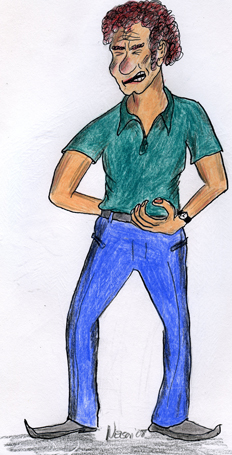
\includegraphics[height=60mm]{corps/chapitre13/img/personnage-claude.jpg}
\end{floatingfigure}

Sey hausse les épaules et raconte tout ce à quoi il vient d’assister dans le bureau de Dauphin : Timothée, Dart Vader, Tropecolo et la violente colère du Flipper.

- Pourquoi que tu me contes ça ?

- Parce que tu es ami avec Timothée et que Dauphin va vraiment se venger. Il a déjà contacté Michaud. Ces salauds sont capables de tout. Ton copain est dans une merde pas possible. Avertis-le et essaie de l’aider à prévenir les coups.

- Comment ?

- Je peux pas trop parler, mais il y a comme un début de piste, le docteur Bellavance.

- Bellavance ? C’est quoi le rapport ?

- Peut-être que s’il voit Timothée être obligé de se défendre contre cette chienlit, il aura le goût de lui dire des choses.

- Quelles choses ?

- Je peux pas t’en dire plus.

Shimoune est sceptique.

- Sérieusement, pourquoi tu viens me dire ça ici, à matin, ma belle p’tite crotte ? Si tu travailles pour le Flipper, t’es aussi pourri que lui non ? Et là en plus, tu viens me le dénoncer. Qu’est-ce qui me dit que tu n’es pas en service commandé ?

- R’garde, tu fais comme tu veux. Je t’ai raconté dans le détail ce qu’il venait de se passer. Si tu me crois pas, questionne Tropecolo, Marie-Odile Tremblay ou monsieur Gagnon. Tu peux aussi aller vérifier ici, en bas, en demandant aux Papyblues. Ceci étant dit, le comique, essaie de ne pas trop t’étouffer dans ta parano de sniffeuse de poudre cheap !

Bouche bée, Shimoune regarde filer Claude Sey.

Et il le restera jusqu’à sa pause de quatorze heures quand Timothée viendra le chercher. En attendant, il tentera de refaire le point. Au terme, son amitié aura pris le dessus sur sa méfiance. Car si son copain est un pourri, s’il est une des créatures de Barrett et du gros Turcotte, comment peut-il prendre le parti d’un vieillard diminué, ayant déjà «un pied dans la tombe», contre Dauphin et Michaud ? Et comment pourrait-il avoir tenu ces propos sur le vieil informaticien, jeudi dernier, lors de la séance du Comité de déontologie ? Est-ce la raison pour laquelle la bande à Turcotte n’entend pas l’aider avec les graves ennuis de sa mère et qu’il doive faire affaire avec le docteur Gagnon ? Est-ce parce que Timothée voudrait prendre ses distances par rapport à l’organisation libérale ? Hum !

Mais d’un autre côté, il se peut aussi que l’équation Mimi Turcotte – Marie Rioux ne soit pas bonne, que ces similitudes ne soient que fortuites, qu’il n’y ait aucun rapport entre le squat de la rue Crouet et le pavillon reclus du Bic. Et c’est connu, des vieux qui sont planqués pour se soustraire aux CRG, il y en a des masses. Si ce n’était pas le cas, il n’y aurait pas les flics du BAG, cette SPCA spécialisée dans le ramassage de vieux. Aussi bien dire qu’il est tout à fait malhonnête de vouloir établir un lien entre ces deux histoires. Les seuls faits qu’on peut vraiment invoquer sont que, d’un côté, il y a Turcotte, sa famille qui échapperait aux CRG en étant cachée dans un bâtiment relevant du MAG, le Flipper et Michaud qui trempent dans cette sale combine, enfin Pete Barrett qui a l’œil ouvert et le bon, ensuite que, d’un autre, il y a Timothée Tardif qui se saigne pour dissimuler ses parents, qui a une mère malade, qui en arrache avec un profiteur du système et qui ne sait plus à quel saint se vouer.

Si tel est le cas, il n’y a plus lieu de confronter ce pauvre diable. Pourquoi l’ennuyer avec des histoires de libéraux qui bafouent leur propre loi ? Mais il l’a soupçonné. Sans compter que sa mère a été associée à l’organisation de Turcotte. Puis, quelque part, le Momo ne lui dit pas tout. Rien n’est moins limpide que ce paquet d’embrouilles; il y a anguille dans les bobettes. Et maintenant qu’il l’a prévenu qu’il avait de l’info pouvant l’intéresser, il aurait l’air étrange de reculer, de tourner son appel téléphonique en plaisanterie, en erreur. Sans oublier cette histoire avec le docteur Bellavance, le sinistre fermier hormonal. Le mieux est sûrement de tout lui raconter, au Timothée, y compris sa suspicion. Un ami que l’on soupçonne un instant du pire et à qui l’on ne se confesse pas d’avoir ainsi pensé, n’est probablement déjà plus un ami, mais une relation mondaine.

- Tiens, si c’est pas le beau Momo, fait-il en le voyant se pointer à la porte de la cafétéria. Moman que t’as pas d’l’air en forme, toi ! Tu r’sembles à un mort qui a mal ressuscité. As-tu bouffé au moins ? J’ai une glacière dans mon char avec des fruits, du fromage, des viandes froides. Y a même un litre de jus d’ananas. Je m’en allais manger ça en prenant le soleil. Ça te tente de partager ?

- Euh … je ne veux pas t’enlever le pain de la bouche.

- Mon de doux ! J’en ai en masse, s’il y en a pour un, il y en a pour deux, Momo ! De toute façon, j’ai une méchante histoire à te conter. Viens !

Les regardant s’en aller, Amédée Chicot se tape la boucle d’oreille et demande la Direction des communications.

- Allô ? J’aimerais parler à Philippe Dauphin.

- C’est à quel sujet ?

- Putain de ta mère, connasse ! Tu lui dis que Chicot a de l’info pour lui, merde, et que ça urge !